\documentclass{article}
\usepackage{bm}
\usepackage{amsmath}
\usepackage{graphicx}
\usepackage{mdwlist}
\usepackage[colorlinks=true]{hyperref}
\usepackage{geometry}
\geometry{margin=1in}
\geometry{headheight=2in}
\geometry{top=2in}
\usepackage{palatino}
%\renewcommand{\rmdefault}{palatino}
\usepackage{fancyhdr}
\usepackage{listings}
%\pagestyle{fancy}
\rhead{}
\lhead{}
\chead{%
  {\vbox{%
      \vspace{2mm}
      \large
      Introduction to Deep Learning M2177.0043 \hfill
\\
      Seoul National University
      \\[4mm]
      Homework \#(\textbf{2})\\
      \textbf{Sanghyeok Park}
    }
  }
}


\usepackage{paralist}

\usepackage{todonotes}
\setlength{\marginparwidth}{2.15cm}

\usepackage{tikz}
\usetikzlibrary{positioning,shapes,backgrounds}

\usepackage{amssymb}

\begin{document}
\pagestyle{fancy}

%% Q1
\section{Q1}

To find all eigenvalues, we can just find all eigenvectors.
When I observe such matrix, I just found eigenvectors easily.
Denote the standard basis as $\{e_i \in \mathbb{R}^p: 1 \leq i \leq p\}$.
At first, vector $[1, 1, \cdots, 1]^T=\sum\limits_{i=1}^{p} e_i$ is eigenvector,
    because $X(\sum\limits_{i=1}^{p} e_i)
    = \sum\limits_{i=1}^{p} Xe_i
    = [(n-1)c+1, (n-1)c+1, \cdots, (n-1)c+1]^T
    = ((n-1)c+1)\sum\limits_{i=1}^{p} e_i$ (Sum of each row is identical!).
So I just found one eigenvalue, $(n-1)c+1$. \\

And I just notice that each pair of rows has only two different element.
For all $1 \leq i < j \leq p$, $e_i - e_j$ could be an eigenvector, because
\begin{align*}
    (X(e_i-e_j))_k &= X_{ki} - X_{kj} \\
    &= (c + \delta_{ki}(1-c)) - (c + \delta_{kj}(1-c)) \\
    &= (1-c)(\delta_{ki} - \delta_{kj}) \\
    &=
    \begin{cases}
        (1-c), & k=i \\
        -(1-c), & k=j \\
        0, & o.w.
    \end{cases}
\end{align*}
Therefore, $X(e_i-e_j) = (1-c)(e_i-e_j)$, so $e_i-e_j$ is eigenvectors.
However, we have to pick linearly independent eigenvectors, so just pick $j=i+1$, i.e.
    $(e_1-e_2), (e_2-e_3), \cdots, (e_{p-1}-e_p)$ (total $p-1$ vectors).
Finally, I just found that all eigenvalue of such eigenvectors is $(1-c)$. \\

In conclusion, eigenvalues are $(1-c)$ ($p-1$ repetition), $(n-1)c+1$.

%% Q2
\section{Q2}

%% Q2-1
\subsection{}
Since $\Sigma$ is real symmetric semi-positive definite matrix,
we can represent $\Sigma = UDU^T$ using SVD,
where $D$ is diagonal matrix and $U$ is unitary matrix.
Let $\bar{X} = X - \mu$ then $\bar{X} \sim N(0, \Sigma)$,
so we just have to find $\bar{X}$. \\

Let $S=UD^{\frac{1}{2}}$ and $\bar{X}=SZ$, then
$E[\bar{X}\bar{X}^T]
= E[SZZ^TS^T]
= SE[ZZ^T]S^T$.
Since samples of $Z$ are independent, non-diagonal element is $0$.
Also each $z_i$ is from $N(0,1)$, so diagonal element is $1$.
Therefore, $SE[ZZ^T]S^T = SIS^T = SS^T = \Sigma$.

Finally, let $X = \mu + SZ$, then $X \sim N(\mu, \Sigma)$.

%% Q2-2
\subsection{}
In this case, we can do diagonalize instead of SVD.
Clearly eigenvectors are $[1,1]^T$ and $[1,-1]^T$,
and corresponding eigenvalues are $1.9$ and $0.1$.
Therefore,
$U =
\begin{bmatrix}
    \frac{1}{\sqrt{2}} & \frac{1}{\sqrt{2}} \\
    \frac{1}{\sqrt{2}} & -\frac{1}{\sqrt{2}}
\end{bmatrix}$.
And
$D =
\begin{bmatrix}
    1.9 & 0 \\
    0 & 0.1
\end{bmatrix}$.
Finally, $\Sigma = UDU^T$. \\

After run following code with python3, image `q2-2.png' appears.

\lstinputlisting[language=Python]{./q2-2.py}

\begin{center}
    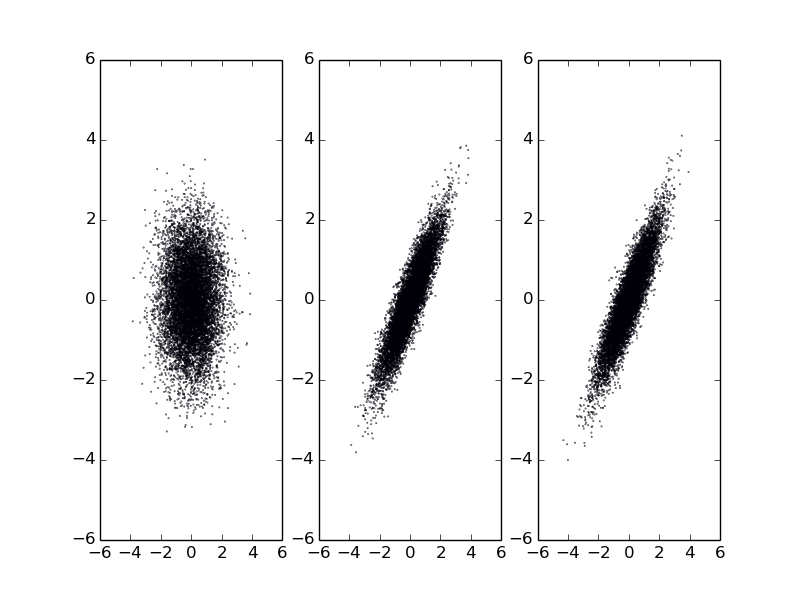
\includegraphics[totalheight=0.5\textheight]{./q2-2.png}
\end{center}

Last two plots look similar!

%% Q3
\section{Q3}

%% Q3-1
\subsection{}
First, let's observe $v_i = \max(0,1-y_i\bold{w}^T\bold{x}_i)$.
If $0 < 1-y_i\bold{w}^T\bold{x}_i$,
$v_i = 1 - y_i\bold{w}^T\bold{x}_i$,
so $\nabla{v_i} = -y_i\bold{x}_i$.
If $0 > 1-y_i\bold{w}^T\bold{x}_i$,
$v_i = 0$, so $\nabla{v_i} = 0$.
On the boundary, just take $\nabla{v_i} = 0$. \\ 

Now, let's calculate $\nabla{||\bold{w}||^2}$.
Let $\bold{w}=[w_1,w_2,\cdots,w_d]^T$.
Then $||\bold{w}||^2 = w_1^2 + w_2^2 + \cdots + w_n^2$,
    so $\frac{\partial{||\bold{w}||^2}}{\partial{w_i}} = 2w_i$.
Therefore, $\nabla{||\bold{w}||^2} = 2\bold{w}$. \\

Finally, we can calculate gradient of the loss function,
\begin{align*}
    \nabla{l(\bold{w})}
    &= \nabla(\frac{1}{n}\sum\limits_{i=1}^n v_i + \frac{\lambda}{2}||\bold{w}||^2) \\
    &= \frac{1}{n}\sum\limits_{i=1}^n \nabla v_i + \lambda\bold{w} \\
    \\
\end{align*}
\begin{align*}
    \nabla v_i =
    \begin{cases}
        -y_i\bold{x}_i, & y_i\bold{w}^T\bold{x}_i < 1 \\
        0 & o.w.
    \end{cases}
\end{align*}

%% Q3-2

\end{document}
